\section*{Recursive Types and Step Indexing}
\subsection*{A motivating introduction to recursive types}
First consider the  following program in the \emph{untyped} lambda calculus:
\[
  \Omega = (\labs{x}{x \; x}) \; (\labs{x}{x \; x})
\]
The interested reader can now try to evaluate the above expression. After a $\beta$-reduction and a substitution we end up with $\Omega$ again, so the evaluation of this expression diverges. Moreover, it is not possible to assign a type to $\Omega$ (again the interested reader may try to verify this by attempting to assign a type). It can hardly come as a surprise that it cannot be assigned a type, as we previously proved that the simply typed lambda calculus is strongly normalizing so if we could assign $\Omega$ a type, then it would not diverge.

To type $\Omega$ we need recursive types. If we are able to type $\Omega$, then we do not have strong normalization (as $\Omega$ is not strongly normalizing). With recursive types we can type structures that are inherently inductive such as lists, trees, and streams.  In an ML like language a declaration of a tree type would look like this:
\begin{lstlisting}
  type tree = Leaf
            | Node of int * tree * tree
\end{lstlisting}
In Java we could define a tree class with an int field and fields for the sub trees:
\begin{lstlisting}
  class Tree {
    int value;
    Tree left, right;
  }
\end{lstlisting}
So we can define trees in our programming languages, but we cannot define them in the lambda calculus. Let us try to find a reasonable definition for recursive types by considering what properties are needed to define trees. We want a type that can either be a node or a leaf. A leaf can be represented by unit (as it here does not carry any information), and a node is the product of an int and two nodes. We put the two together with the sum type, as it is:
\[
  tree = 1 + (int * tree * tree)
\]
This is what we want, but we cannot specify this. We try to define $tree$, but $tree$ appears on the right hand side, which is self-referential. Instead of writing $tree$ we use a type variable $\alpha$:
\begin{align*}
  \alpha &= 1 + (int \times \alpha \times \alpha) \\
         &= 1 + (int \times (int \times \alpha \times \alpha) \times (int \times \alpha \times \alpha)) \\
  &\vdots
\end{align*}
All the sides of the above equations are equal, and they are all trees. We could keep going and get an infinite system of equations. If we keep substituting the definition of $\alpha$ for $\alpha$ we keep getting bigger and bigger types. All of the types are trees, and all of them are finite. If we take the limit of this process, then we end up with an infinite tree, and that tree is the tree we conceptually have in our minds. So what we need is the fixed point of the above equation.

Let us define a recursive function who's fixed point we want to find:
\[
F = \lambda \alpha :: type. 1 + (int \times \alpha \times \alpha)
\]
We want the fixed point which by definition is $t$ such that
\[
  t = F(t)
\]
So we want
\[
  tree = F(tree)
\]
The fixed point of this function is written:
\[
  \mu \alpha.\; F(\alpha)
\]
Here $\mu$ is a fixed point type constructor. As the above is the fixed point, then by definition it should be equal to $F$ applied to it:
\[
  \mu \alpha.\; F(\alpha) = F(\mu \alpha.\; F(\alpha))
\]
Now let us make this look a bit more like types by substituting $F(\alpha)$ for $\tau$. 
\[
  \mu \alpha.\; \tau = F(\mu \alpha.\; \tau) 
\]
The right hand side is really just $\tau$ with $\mu \alpha. \; \tau$ substituted with $\tau$:
\[
  \mu \alpha.\; \tau = \tau[\mu \alpha. \; \tau / \alpha]
\]
We are going to introduce the recursive type $\mu \alpha.\; \tau$ to our language. When we have a recursive type we can shift our view to an expanded version $\tau[\mu \alpha. \; \tau / \alpha]$ and contract back to the original type. Expanding the type is called $\unfold$ and contracting is is called $\fold$.
\[
\begin{tikzpicture}[->,>=stealth',shorten >=1pt,auto,node distance=3cm,
  thick,main node/.style={rectangle}]

  \node[main node] (1) {$\mu\alpha.\; \tau$};
  \node[main node] (2) [right of=1] {$\tau[\mu \alpha. \; \tau / \alpha]$};

  \path[every node/.style={font=\sffamily\small}]
    (1) edge [bend left] node [above] {$\unfold$} (2)
    (2) edge [bend left] node [below] {$\fold$} (1);
\end{tikzpicture}
\]
With recursive types in hand we can now define our tree type:
\[
  tree \eqdef \mu \alpha. \; 1 + (int \times \alpha \times \alpha)
\]
When we want to work with this, we would like to be able to get under the $\mu$. Say we have $e : tree$ that is an expression $e$ with type $tree$, then we want to be able to say whether it is a leaf or a node. To do so we unfold the type to get the type where $\alpha$ has been substituted with the definition of $tree$ and the outer $\mu\alpha.$ has been removed. With the outer $\mu\alpha.$ gone we can match on the sum type to find out whether it is a leaf or a node. When we are done working with the type we can fold it back to the original tree type.
\[
\begin{tikzpicture}[->,>=stealth',shorten >=1pt,auto,node distance=3cm,
  thick,main node/.style={rectangle}]

  \node[main node] (1) {$tree=\mu\alpha.\; 1+(int \times \alpha \times \alpha)$};
  \node[main node] (2) [right of=1,xshift=5cm] {$1+(int \times (\mu\alpha.\; 1+(int \times \alpha \times \alpha)) \times (\mu\alpha.\; 1+(int \times \alpha \times \alpha)))$};

  \path[every node/.style={font=\sffamily\small}]
    (1) edge [bend left=10] node [above] {$\unfold$} (2)
    (2) edge [bend left=10] node [below] {$\fold$} (1);
\end{tikzpicture}
\]
This kind of recursive types is called iso-recursive types, because there is an isomorphism between a $\mu\alpha. \; \tau$ and its unfolding $\tau[\mu\alpha.\; \tau / \alpha]$. 

\subsection*{Simply typed lambda calculus extended with $\mu$}
STLC extended with recursive types is defined as follows:
\begin{align*}
  \tau &::= \dots \vbar \mu \alpha. \; \tau \\
  e    &::= \dots \vbar \fold \; e \vbar \unfold \; e \\
  v    &::= \dots \vbar \fold \; v\\
  E    &::= \dots \vbar \fold \; E \vbar \; \unfold \; E
\end{align*}
\[
\unfold \; (\fold \; v) \evalto v
\]
\[
\TFold \hspace{2cm} \TUnfold
\]
With this we could define the type of an integer list as:
\[
int\; list \eqdef \mu\alpha.\; 1 + (int \times \alpha)
\]
%TODO: Typing omega
\begin{comment}
\[
  \Omega = (\tlabs{x}{\mu\alpha.\; \tarrow{\alpha}{\tau}}{(\unfold \; x) \; x}) 
\]
\end{comment}

\subsection*{Step-indexing, logical relations for recursive types}
In a naive first attempt to make the value interpretation we could write something like
\[
  \vpred{\mu\alpha. \; \tau} = \{\fold \; v \vbar \unfold \; (\fold \; v) \in \epred{\sub{\tau}{\mu\alpha.\;\tau}{\alpha}} \}
\]
We can simplify this slightly; first we use the fact that $\unfold \; (\fold \; v)$ reduces to $v$. Next, we use the fact that $v$ must be a value and the fact that we want $v$ to be in the expression interpretation of $\tau[\mu \alpha. \; \tau / \alpha]$. By unfolding the definition of the expression interpretation we conclude that it suffices to require $v$ to be in the value interpretation of the same type. We then end up with the following definition:
\[
  \vpred{\mu\alpha. \; \tau} = \{\fold \; v \vbar v \in \vpred{\sub{\tau}{\mu\alpha.\;\tau}{\alpha}} \}
\]
This gives us a well-foundedness issue. The value interpretation is defined by induction on the type, but $\sub{\tau}{\mu\alpha.\;\tau}{\alpha}$ is not a structurally smaller type than $\mu\alpha. \; \tau$. 

To solve this issue we index the interpretation by a natural number, $k$, which we write as follows:
\[
  \vpres{\tau} = \{v \vbar \dots \}
\]
Hence, $v \in \vpres{\tau}$ is read as ``$v$ belongs to the interpretation of $\tau$ for $k$ steps.'' We interpret this in the following way: given a value that we run run for $k$ or fewer steps (as in the value is used in some program context for fewer than $k$ steps) then we will never notice that it does not have type $\tau$. If we use the same value in a program context that wants to run for more than $k$ steps, then we might notice that it does not have type $\tau$ which means that we might get stuck. This gives us an approximate guarantee.

We use this as an inductive metric to make our definition well-founded, so we define the interpretation on induction on the step-index followed by an inner induction on the type structure. Let us start by adding the step-index to our existing value interpretation:
\begin{align*}
  \vpres{bool} &= \{\true,\false\} \\
  \vpres{\tarrow{\tau_1}{\tau_2}} &= \{\tlabs{x}{\tau_1}{e} \vbar \forall j \leq k. \; \forall v \in \vpres[j]{\tau_1}. \; \sub{e}{v}{x} \in \epres[j]{\tau_2} \}
\end{align*}
$\true$ and $\false$ are in the value interpretation of $bool$ for any $k$, so $\true$ and $\false$ will for any $k$ look like it has type $bool$. To illustrate how to understand the value interpretation of $\tarrow{\tau_1}{\tau_2}$ please consider the following time line:  \\
\begin{center}
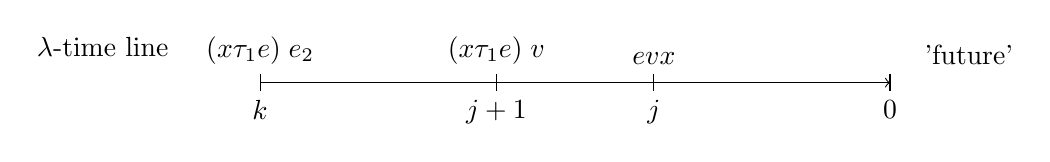
\begin{tikzpicture}
    % draw horizontal line   
    \draw[->] (0,0) -- (8,0);

    % draw vertical lines
    \foreach \x in {0,3,5,8}
      \draw (\x cm,3pt) -- (\x cm,-3pt);

    % draw nodes
    \draw (-2,0) node[below=3pt] {  } node[above=6pt] {$\lambda$-time line};
    \draw (0,0) node[below=3pt] {$k$} node[above=3pt] {$(\tlabs{x}{\tau_1}{e}) \; e_2$};
    \draw (3,0) node[below=3pt] {$ j+1 $} node[above=3pt] {$(\tlabs{x}{\tau_1}{e})\; v $};
    \draw (4.3,0) node[below=3pt] {$   $} node[above=3pt] {$ \evalto $};    
    \draw (5,0) node[below=3pt] {$ j $} node[above=3pt] {$ \sub{e}{v}{x} $};
    \draw (8,0) node[below=3pt] {$ 0 $} node[above=3pt] {$  $};
    \draw (9,0) node[below=3pt] {$   $} node[above=3pt] { 'future' };
  \end{tikzpicture}
\end{center}
Here we start at index $k$ and as we run the program we use up steps until we at some point reach 0 and run out of steps. At step $k$ we are looking at a lambda. A lambda is used by applying it, but it is not certain that the application will happen right away. We only do a $\beta$-reduction when we try to apply a lambda to a value, but we might be looking at a context where we want to apply the lambda to an expressions, i.e.\ $(\tlabs{x}{\tau_1}{e})\; e_2$. We might use a bunch of steps to reduce $e_2$ down to a value, but we cannot say how many. So say that sometime in the future have fully evaluated $e_2$ to $v$ and say that we have $j+1$ steps left at this time, then we can do the $\beta$ reduction which gives us $\sub{e}{v}{x}$ at step $j$. % If we ever hit 0 steps, then all bets are off. the value can have any type.

We can now define the value interpretation of $\mu\alpha. \; \tau$:
\[
  \vpres{\mu\alpha.\; \tau} = \{\fold \; v \vbar \forall j < k. \; v \in \vpres[j]{\sub{\tau}{\mu\alpha.\;\tau}{\alpha}} \}
\]
This definition is like the one we previously proposed, but with a step-index. This definition is well-founded because $j$ is required to be \emph{strictly} less than $k$ and as we define the interpretation on induction over the step-index this is indeed well founded. We do not define a value interpretation for type variables $\alpha$, as we have no polymorphism yet. The only place we have a type variable at the moment is in $\mu\alpha. \; \tau$, but in the interpretation we immediately close off the $\tau$ under the $\mu$, so we will never encounter a free type variable.

Finally, we define the expression interpretation:
\[
  \epres{\tau} = \{e \vbar \forall j < k. \; \forall e'. \; e \evaltos[j] e' \pand \irred(e') \; \implies \; e' \in \vpres[k-j]{\tau}\}
\]
To illustrate what is going on here consider the following time line: \\
\begin{center}
\begin{tikzpicture}
    % draw horizontal line   
    \draw[->] (0,0) -- (4,0);

    % draw vertical lines
    \foreach \x in {0,2,4}
      \draw (\x cm,3pt) -- (\x cm,-3pt);

    % draw nodes
    \draw (0,0) node[below=3pt] {$k$} node[above=3pt] {$e$};
    \draw (1,0) node[below=3pt] {$ $} node[above=3pt] {$\evalto \evalto \evalto \evalto$};
    \draw (2,0) node[below=3pt] {$k-j$} node[above=3pt] {$e'$};
    \draw (4,0) node[below=3pt] {$0$} node[above=3pt] {$  $};

    % brace
    \draw [decorate,decoration={brace,amplitude=10pt,mirror}]
    (0,-0.6) -- (2,-0.6) node [black,midway,yshift=-0.5cm] 
          {\footnotesize $j$};
\end{tikzpicture}
\end{center}
We start with an expression $e$, then we take $j$ steps and get to expression $e'$. At this point if $e'$ is irreducible, then we want it to belong to the value interpretation of $\tau$ for $k-j$ steps. We use a strict inequality because we do not want to hit 0 steps. If we hit 0 steps, then all bets are off.%TODO: why are all bets off?

We also need to lift the interpretation of type environments to step-indexing:
\begin{align*}
  \gpres{\mtenv} & = \{\emptyset \} \\
  \gpres{\Gamma, x : \tau} & = \{ \gamma[x \mapsto v] \vbar \gamma \in \gpres{\Gamma} \pand v \in \vpres{\tau} \}
\end{align*}
Finally we are in a position to lift the definition of semantic type safety to one with step-indexing.
\[
  \Gamma \models e : \tau \eqdef \forall k \geq 0. \; \forall \gamma \in \gpres{\Gamma} \; \implies \gamma(e) \in \epres{\tau}
\]
To actually prove type safety we do it in two steps. First we state and prove the fundamental theorem:
\begin{stlcmufundprop}[Fundamental property] ~\\
  If $\Gamma \vdash e : \tau$ then $\Gamma \models e : \tau$.
\end{stlcmufundprop}
When we have proven the fundamental theorem we prove that it entails type safety.
\[
\circled{b} \quad \mtenv \models e : \tau \implies \safe(e)
\]
Thanks to the way we defined the logical predicate this second step should be trivial to prove.

To actually prove the fundamental theorem, which is the challenging part, we need to prove a monotonicity lemma:
\begin{monotonicity}[Monotonicity] ~\\
  If $v\in \vpres{\tau}$ and $j \leq k$  then $v \in \vpres[j]{\tau}$.
\end{monotonicity}
\begin{proof}
The proof is by case on $\tau$.
\case{$\tau = bool$}
assume $v \in \vpres{bool}$ and $j \leq k$, we then need to show $v \in \vpres[j]{bool}$. As $v \in \vpres{bool}$ we know that either $v= \true$ or $v=\false$. If we assume $v=\true$, then we immediately get what we want to show, as $\true$ is in $\vpres[j]{bool}$ for any $j$. Likewise for the case $v=\false$.
\case{$\tau = \tarrow{\tau_1}{\tau_2}$}
assume $v \in \vpres{\tarrow{\tau_1}{\tau_2}}$ and $j \leq k$, we then need to show $v \in \vpres[j]{\tarrow{\tau_1}{\tau_2}}$. As $v$ is a member of $\vpres{\tarrow{\tau_1}{\tau_2}}$ we can conclude that $v = \tlabs{x}{\tau_1}{e}$ for some $e$. By definition of $v \in \vpres[j]{\tarrow{\tau_1}{\tau_2}}$ we need to show $\forall i \leq j. \forall v' \in \vpres[i]{\tau_1}.\; \sub{e}{v'}{x} \in \epres[i]{\tau_2}$. Suppose $i \leq j$ and $v' \in \vpres[i]{\tau_1}$, we then need to show $\sub{e}{v'}{x} \in \epres[i]{\tau_2}$.

By assumption we have $v \in \vpres{\tarrow{\tau_1}{\tau_2}}$ which gives us $\forall n \leq k. \; \forall v' \in \vpres[n]{\tau_1}.\; \sub{e}{v'}{x} \in \epres[n]{\tau_2}$. From $j \leq k$ and $i \leq j$ we get $i \leq k$ by transitivity. We use this with $v' \in \vpres[i]{\tau_1}$ to get $\sub{e}{v'}{x} \in \epres[i]{\tau_2}$ which is what we needed to show.
\case{$\tau = \mu \alpha.\; x$}
assume $v \in \vpres{\mu\alpha. \; \tau}$ and $j \leq k$, we then need to show $v \in \vpres[j]{\mu\alpha. \; \tau}$. From $v$'s assumed membership of the value interpretation of $\tau$ for $k$ steps we conclude that there must exist a $v'$ such that $v = \fold \; v'$. If we suppose $i<j$, then we need to show $v' \in \vpres[i]{\subst{\tau}{\mu\alpha.\; \tau}{\alpha}}$. From $i<j$ and $j \leq k$ we can conclude $i < k$ which we use with $\forall n < k.\; v' \in \vpres[n]{\subst{\tau}{\mu\alpha.\; \tau}{\alpha}}$, which we get from $v \in \vpres{\mu\alpha. \; \tau}$, to get $v' \in \vpres[i]{\subst{\tau}{\mu\alpha.\; \tau}{\alpha}}$.
\end{proof}
\begin{comment}
  \begin{lemma}[Substitution]
    Let $e$ be syntactically well-formed term, let $v$ be a closed value and let $\gamma$ be a substitution that map term variables to closed values, and let $x$ be a variable not in the domain of $\gamma$, then
    \[
    \extsub{\gamma}{x}{v}(e) = \subst{\gamma(e)}{x}{v}
    \]
  \end{lemma}
\end{comment}
\begin{proof}[Proof (Fundamental Property)]
Proof by induction over the typing derivation.
\case{\TFold} \\~
We need to show 
\newcommand{\mat}{\ensuremath{\mu\alpha.\tau}}
v\[
  \Gamma \models \fold \; e : \mat
\]
So suppose we have $k \geq 0$ and $\gamma \in \gpres{\mat}$, then we need to show $\gamma(\fold\; e) \in \epres{\mat}$ which amounts to showing $\fold\; \gamma(e) \in \epres{\mat}$.

So suppose that $j<k$ and that $\fold\; \gamma(e) \evaltos[j] e'$ and $\irred(e')$, then we need to show $e' \in \vpres[k-j]{\mat}$. As we have assumed that $\fold\; \gamma(e)$ reduces down to something irreducible and the operational semantics of this language are deterministic we know that $\gamma(e)$ must have evaluated down to something irreducible. We therefore know that $\gamma(e) \evaltos[j_1] e_1$ where $j_1 \leq j$ and $\irred(e_1)$.
Now we use our induction hypothesis:
\newcommand{\tsub}{\ensuremath{\sub{\tau}{\mat}{\alpha}}}
\[
  \Gamma \models e : \tsub
\]
We instantiate this with $k$ and $\gamma \in \gpres{\Gamma}$ to get $\gamma(e) \in \epres{\tsub}$. Which we then can instantiate with $j_1$ and $e_1$ for get $e_1 \in \vpres[k-j_1]{\tsub}$. Now let us take a step back and see what happened: We started with a $\fold\; \gamma(e)$ which took $j_1$ steps to $\fold\; e_1$. We have just shown that this $e_1$ is actually a value as it is in the value interpretation of $\vpres[k-j_1]{\tsub}$. To remind us $e_1$ is a value let us henceforth refer to it as $v_1$. We further know that $\fold\; \gamma(e)$ reduces to $e'$ in $j$ steps and that $e'$ was irreducible. $\fold\; v_1$ is also irreducible as it is a value and as our language is deterministic it must be the case that $e' = \fold\; v_1$ and thus $j = j_1$. Our proof obligation was to show $e' = \fold \; v_1 \in \vpres[k-j]{\mat}$ to show this suppose we have $l < k-j$ (this also gives us $l < k-j_1$ as $j = j_1$). We then need to show $v_1 \in \vpres[l]{\tsub}$, we obtain this result from the monotonicity lemma using $\vpres[k-j_1]{\tsub}$ and $l < k-j_1$.
\end{proof}

The list example from the previous lecture used the sum type. Sums are a straight forward extension of the language. The extension of the value interpretation would be:
\[
  \vpres{\tau_1 + \tau_2} = \{\inl \; v_1 \vbar v_1 \in \vpres{\tau_1}\} \cup 
                            \{\inr \; v_2 \vbar v_2 \in \vpres{\tau_2}\}
\]
We can use $k$ directly or $k$ decremented by one. It depends on whether we want casing to take up a step. Either way the definition is well-founded. 

\subsection*{Exercises}
\begin{enumerate}
\item Do the lambda and application case of the \emph{Fundamental Property} theorem.%Specify in what proof, probably fundemental property
\item Try to prove the \emph{monotonicity} lemma where the definition of the value interpretation has been adjusted with:
\[
\vpres{\tarrow{\tau_1}{\tau_2}} = \{\tlabs{x}{\tau_1}{e} \vbar \; \forall v \in \vpres{\tau_1}. \; \sub{e}{v}{x} \in \epres{\tau_2} \}
\]
This will fail, but it is instructive to see how it fails.
\end{enumerate}
